\chapter{Opracowanie wyników}

Rozdział ten zawiera analizę wyników opisanego w~części~\ref{cha:implementacja}.


\section{Wielkość błędu}
asdasd

\section{Warianty opadu}

\section{Analiza wrażliwości na posterunki opadowe}
W~tej części przeprowadzono wpływ wyłączenia wskazanego posterunku opadowego (ograniczono się do wybory punktów zawartych w granicach wskazanej zlewni) na wynik działania omawianej metody. Pozwala to znaleźć odpowiedź na pytanie: \textit{Czy sieć istniejących posterunków opadowych jest wystarczająca?}, a~to pomoże podejmować decyzje o~zwiększaniu ilości owych posterunków bądź przeniesieniu w~inną lokalizację.

Rysunek~\ref{fig:identyfikatory} przedstawia identyfikatory wykluczanych z~analizy punktów, natomiast wiersze tabeli prezentują rezultat działania programu bez zadanego punktu.

\begin{figure}[ht]
	\centering
	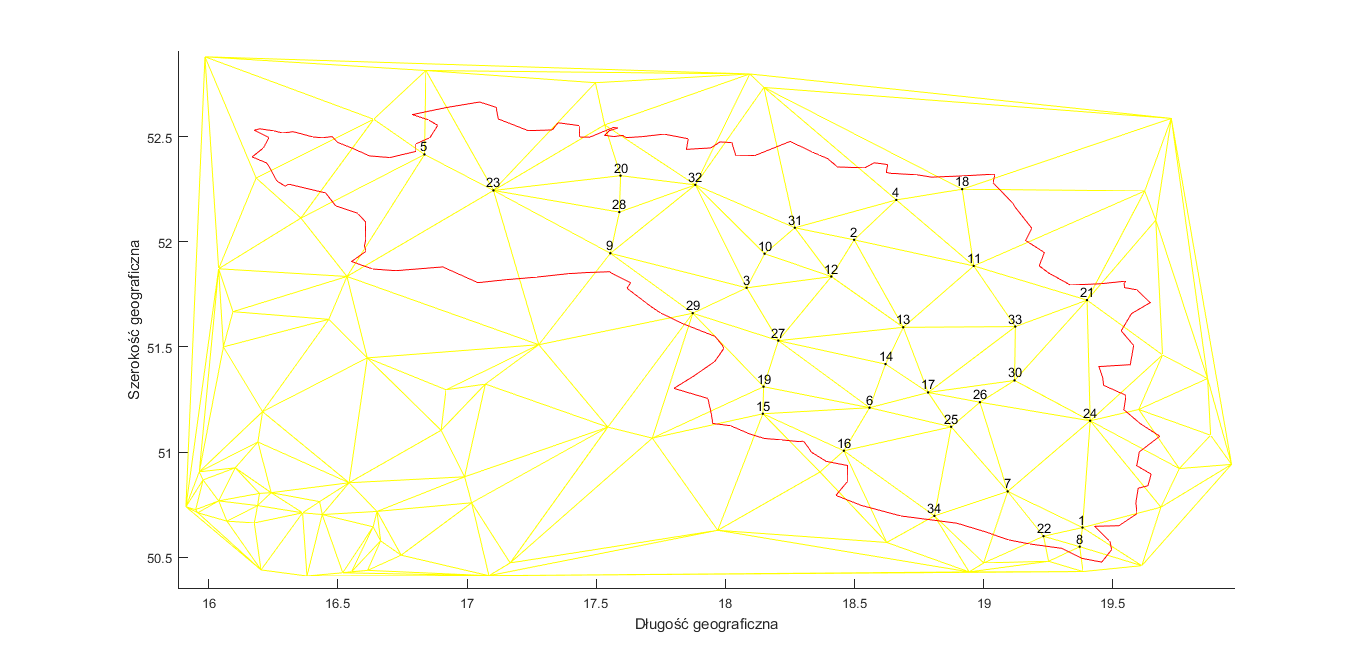
\includegraphics[width=1\linewidth]{identyfikatory_punktow}
	\label{fig:identyfikatory}
	\caption{Identyfikatory posterunków wewnątrz zlewni}
\end{figure}

\subsection{Wniosek}